\chapter{Reinforcement Learning}\label{ch:RL}

Here I'll go over the fundamentals of Neural Network and Machine Learning as well as the some applications and practical applications. Then I'll go over the fundamentals of Reinforcement Learning from the typical formalism to some of the latest methods and algorithms.

Before we even go over neural network, I do believe in having a strong foundation in the subject and a clear mathematical formalism. This allows for a subject's mathematical description of methods to speak to us in a clear and understandable language forming a clear picture.

\section{Introductory Mathematics}

\subsection{Formalism}

In this paper, I heavily rely on the formalism typically expressed in linear algebra textbooks. This allows me to relay the most important information, intuitively, while preserving exactness.

To describe a scalar, mathematically, a standard letter a used. For instance $a=1$, where I assign the variable $a$ the scalar value of $1$. To describe a vector, an arrow is placed above a variable to denote it as a vector, $\vec{v}=\vec{0}$ denotes a variable $\vec{v}$ assigned the zero vector. A vector can be described as an element of n-dimensional Euclidean Space where each element of the vector denotes an axis of said space. $$\vec{x}=\begin{bmatrix}1 & 2 & 3\end{bmatrix}$$ is an example vector in 3 dimensional euclidean space. This same vector is denoted as a row-wise vector, where all the elements of the vector are on a single row, a column-wise vector would look like $$\vec{x}=\begin{bmatrix}1 \\ 2 \\ 3\end{bmatrix}.$$ The significance of the distinctions between a row-wise and column-wise vector are show when going over the matrix as in some operations they have different results and making a distinction matters. From now on when a vector is shown and is not other wise said assume the vector is in column-wise form. 

Another form that a vector can be expressed in is via summation notation. In this notation, we must first define the following unit vectors, $$\hat{r}_1=\begin{bmatrix}1 \\ 0 \\ \vdots \\ 0\end{bmatrix},\hat{r}_2=\begin{bmatrix}0 \\ 1 \\ \vdots \\ 0\end{bmatrix},\dots,\hat{r}_n=\begin{bmatrix}0 \\ 0 \\ \vdots \\ 1\end{bmatrix} .$$ Each element of said vector can then be denoted as $$\vec{x}=x_1 \hat{r}_1 + x_2 \hat{r}_2 + \dots + x_n \hat{r}_n$$ and finally using sigma notation, $$\vec{x}=\sum_{i=1}^n x_i \hat{r}_i.$$ This notation is important to properly display information and proofs that would be difficult to display using the previously show forms. One example proof is the proof for the vector's associativity axiom, $\vec{u}+(\vec{v}+\vec{w})=(\vec{u}+\vec{v})+\vec{w}$.
\begin{proof}
\begin{align*}
\vec{u}+(\vec{v}+\vec{w})&=(\vec{u}+\vec{v})+\vec{w} \\
&=\bigg(\sum_{i=1}^nu_i \hat{r}_i+\sum_{j=1}^n v_j \hat{r}_j\bigg)+\sum_{k=1}^n w_k \hat{r}_k\\
&=\sum_{i=1}^n (u_i\hat{r}_i + v_i\hat{r}_i) + w_i\hat{r}_i\\
&=\sum_{i=1}^n \big((u_i + v_i) + w_i\big)r_i\\
&=\sum_{i=1}^n \big(u_i+(v_i+w_i)\big)r_i&\text{scalar's associativity}\\
&=\vec{u}+(\vec{v}+\vec{w})
\end{align*}
\end{proof}

\subsection{Matrix Operations}

In this section, I will go over the common matrix operations that are used in Machine Learning. Firstly, a matrix is basically a table of mathematical expression or numbers arranged in columns and rows. For example, $$A=\begin{bmatrix} 1 & 2 \\ 3 & 4 \end{bmatrix}.$$ Both row vectors and column vectors can be seen as matrices with a single row or a single column. In this paper, when ever a letter is capitalized it means that it represent a matrix. When a matrix is show as $[A]_{ij}$ this means we are talking about the element in the $i$th row and the $j$th column.

\subsubsection{Component-wise Operations}

Component wise operations like multiplication, addition, and subtraction can be denoted on a per component basis. $$[A\square B]_{ij}=[A]_{ij} \square [B]_{ij}$$

The $\square$ symbols represent the different possible component-wise operations like multiplication, add, subtraction, and even division.

\subsubsection{Matrix Multiplication}

Matrix Multiplication is the most heavily used operation in Machine Learning. It's definition is simple, in summation notation, $$[AB]_{ij}=\sum_{k=1}^n [A]_{ik}[B]_{kj}.$$

\subsubsection{Matrix Transpose}

The transpose operation is also used extensively. It is defined as $$[A^T]_{ij}=[A]_{ji}.$$

\subsection{Dot Product}

Both single rowed, and single columned matrices are vectors, which means we can borrow some of the operations, for instance, the component-wise operations.

The Dot Product is defined as $$\vec{a}\cdot \vec{b}=\sum_{i=1}^n a_i b_i.$$ Notice, the Dot Product basically is Matrix Multiplication between two vectors, one in the form of a row vector and the other as a column vector. 

\begin{proof}
\begin{align*}
\vec{a}\cdot \vec{b}&=\vec{a}\vec{b}^T\\
&=\begin{bmatrix}a_1 & a_2 & \dots \end{bmatrix}
\begin{bmatrix}b_1 \\ b_2 \\ \vdots \end{bmatrix}\\
&=\sum_{i=1}^na_i b_i \\
&=\vec{a}\cdot \vec{b}
\end{align*}
\end{proof}

\section{Neural Networks}

The history of neural networks goes back to the 1940 but was really popularized with the perceptron in the 50s and 60s where the perceptron was implemented on an IBM 704.

\subsection{Perceptrons}

In the simplest of thinking a perceptron simply is a single-layer Neural Network and one of earliest forms of a Neural Network, \cite{rosenblatt_1958}. It basically is a piecewise function where a weights $w$ and bias $b$ determine the output. $$f(\vec{x})=\begin{cases}
1 \mbox{ if } \vec{w}\cdot \vec{x}+b>0 \\
0 \mbox{ otherwise }
\end{cases}$$ Where $\vec{w}$  is the weight vector, $b$ is the bias, and $x$ is the input vector.  Perceptrons are a powerful concept since n-Dimensional clusters can be linearly separated. A great example where perceptrons are extremely helpful is with logical operators. A single perceptron can mimic most logical operators except for XOR; Multiple perceptrons can mimick XOR. Since the perceptron is a linear classifier, the perceptron will fail if a cluster is not linearly separable. 

One example of a logical operator that a perceptron can mimic is the AND function. The AND function is only true when both both inputs are true. Let true be one and false be zero, then if $\vec{w}=\begin{bmatrix}1 \\ 1\end{bmatrix}$ and $b=-1.5$ then the perceptron will only output one when both inputs are one.

\subsection{Feed-forward Neural Networks}

We can classify Feed-forward Neural Networks into several categories. One of these categories, the simplest, is the Single Neuron Single Input Network. 
$$a(x)=f(wx + b)|_{w.b}$$
$w$ and $b$ are weight constants, and $f$ is a transfer function that can be linear or non-linear function and whose purpose is to turn input information into output info—for example, turning input data into 0s and 1s using the piecewise function, thereby turning into a perceptron. A Single Neuron Multiple Input Neural Network is the next simplest. Here, the Neural Network can be described similarly as the perceptron except for the additional function variable, $$a(\vec{x})=f(\vec{w}\cdot \vec{x}+b).$$ The next most straightforward form of the Neural Network is the Neural Network layer, where a Neural Network has multiple inputs and multiple neurons, resulting in multiple output values, or an output vector. 
$$\vec{a}(\vec{x})=\vec{f}(W\vec{x}+\vec{b})$$ Where $W\vec{x}$ is the Matrix-Vector Multiplication, $$[W\vec{x}]_i=\sum_{j=1}^n [W]_{ij}[\vec{x}]_{j}.$$ 

A Feed-Forward Neural Network's basic anatomy is then an initial input layer, an output layer, and any number of hidden layers. Using the equations so far, it is then possible to build these FNNs. Let us consider this FNN with an arbitrary number of layers, $m$, and an arbitrary number of Neurons per layer. The layers are then 
\begin{align*}
\vec{a}_1 &= f_1(W_1\vec{x} +\vec{b}_1 )\\
&\vdots\\
\vec{a}_i &= f_i(W_i\vec{a}_{i-1}+\vec{b}_i)\\
&\vdots\\
\vec{a}_m &= f_m(W_m\vec{a}_{m-1}+\vec{b}_m)\\
\end{align*}

\begin{figure}
	\centering
	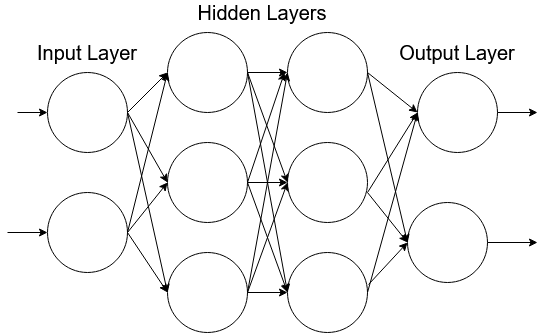
\includegraphics[scale=0.55]{NNDiagram}
	\caption{A diagram of a Feed Forward Neural Network with an input layer, hidden layers, and an output layer.}
	\label{fig:NNDiagram}
\end{figure}

\subsection{Convolutional Neural Networks}

\subsection{Loss and Activation Functions}

Loss and Activation functions are an essential part of the Neural Network Architecture. The Loss function is the metric by which Neural Networks are evaluated and trained. On the other had, activation functions allow for the Neural Network's flexibility by giving it non-linearity.

The activation function, in the context of the definition above, is $f_i$. These functions, as I have said before, allow for the non-linearity of the Neural Network. A couple of typically used functions is the cosine, tangent, ReLU, Leaky ReLU, the logistic function, and many others. Each of these different functions has different properties, which makes each function perfect for a particular scenario. For example, in a Convolutional Neural Network, which typically is deep or has many layers, the ReLU or Leaky ReLU function is used as they help prevent the vanishing or exploding gradient problems.

Loss functions turn the raw output of a neural network into something trainable by an optimization algorithm. These loss functions measure the error between the desired value and the value produced by a neural network. One might ask, why not use the accuracy to train? Unfortunately, since the accuracy function is not differentiable, it cannot be used as a loss function and train a neural network. Some typical functions are the mean square error or the l2-loss, the l1-loss, the hinge loss function, the cross-entropy loss, the negative log-likelihood, and many more.

\section{Back-Propagation, SGD, and ADAM}

Back-Propagation is a specific case of Automatic Differentiation (AD). AD is a Differentiation technique that takes advantage of the fact that computers evaluate expression sequentially. This fact allows for the repeated application of the chain rule. While being similar to both Symbolic Differentiation and Numerical Differentiation, it is neither. Both classical methods of differentiation are comparatively slow at calculating the gradient to complicated functions. 

The chain rule, in calculus, is a formula to calculate the derivative of a composite function. If two functions, $f$ and $g$ are composite, that composite function is $h$, and $h$'s dependent variable is $x$ then the chain rule defined as 
$$\frac{dh(x)}{dx}=\frac{d}{dx}(f(g(x)))=\frac{df}{dg}\bigg|_{g(x)}\cdot\frac{dg}{dx}\bigg|_{x}.$$ Forwards and Backwards accumulation of the computation graph is allowed using the chain rule. Many great tools exist to calculate this create and use these computation graphs via a GradientTape to calculate the gradient of arbitrary functions like PyTorch or Tensorflow python libraries. These library's GradientTape allows for the easy calculation of the gradient without laborious manual calculation of Back-propagation.

\subsection{Stochastic Gradient Descent}

The Stochastic Gradient Descent (SGD) is a stochastic approximation of the Gradient Descent algorithm that finds the minimum or optimizes a function. In the SGD algorithm, calculate the gradient resulting from a single randomly picked sample, then multiply it by a learning rate, hyper-parameter between 0 and 1, then add it to the weights to biases. $$\vec{w}=\vec{w}-\gamma\nabla \vec{f}(\vec{x})$$ Applying Back-propagation and SGD to Neural Networks if the mean square error is used as the loss-function. results in 
\begin{align*}
W_{m}(k+1)&=W_{m}(k)-\gamma \vec{s}_m (\vec{a}_{m-1})^T\\
\vec{b}_m(k+1)&=\vec{b}_{m}(k)-\gamma \vec{s}_m
\end{align*} where
\begin{align*}
s_{M}&=-2\dot{F}_M(\vec{n}_M)(\vec{t}-\vec{a})\\
s_m&=\dot{F}_m(\vec{n}_m)(W_{m+1})^T s^{m+1}\\
\dot{F}(\vec{n}_m)&=I\dot{f}(\vec{n}_m)^T,
\end{align*} $I$ is the square identity matrix, and $m=M-1,\dots, 2, 1$ or for each layer, in reverse. As said before, the $s_M$ variable presented here is for the mean squared error loss function \cite{hagan_demuth_beale_jesus_orlando_de_2014}.

\subsection{ADAM}

What makes the Adam algorithm so popular is its robustness to changes in its hyper-parameters. It does this by keeping a single learning rate and an adaptive learning rate for different parameters calculated from a first and second gradient moments or moving averages of the gradient. Adam combines two algorithms. AdaGrad and RMSprop, combining their advantages over SGD. It has a couple of extra hyper-parameters, including $\beta_1$, $\beta_2$, and $\epsilon$. $\beta_1$ and $\beta_2$ are hyper-parameters that deal with the two moments, and $\epsilon$ improves numerical stability \cite{kingma_ba_2017}. It is calculated by first calculating the current running average, \begin{align*}
	k_m(t+1)&\leftarrow \beta_1 k_m(t)+(1-\beta_1)\nabla \vec{f}(\vec{x})\\
	v_m(t+1)&\leftarrow \beta_2 v_m(t)+(1-\beta_2)(\nabla \vec{f}(\vec{x}))^2\\
	\hat{k}_m&=\frac{k_m(t+1)}{1-\beta_1^{t+1}}\\
	\hat{v}_m&=\frac{v_m(t+1)}{1-\beta_2^{t+1}},
\end{align*} then update the weights, 
$$w_m(t+1)\leftarrow w_m(t)-\gamma\frac{\hat{k}_m}{\sqrt{\hat{v_m}}+\epsilon}.$$

\section{Reinforcement Learning}

According to "Artificial Intelligence: A Modern Approach" by Russel and Norvig an agent as "anything that can be viewed as perceiving its environment through sensors and acting upon that environment through actuators." For instance, an autonomous car will have the roads, and the area around the roads as the environment perceives through the various IR, radar, and visual sensors around the car. The autonomous car will interact with the environment through its various actuators, the accelerator, the brake, and the steering. 

In terms of the environment, I will describe the agent as a satellite that is orbiting a pseudo-earth with a heavier atmosphere, to simulate an accelerated orbital decay. The orbital decay is accelerated because the orbital decay forces are relatively minute, so creating an agent in a reasonable amount of time with a reasonable amount of computational resources is done. Of course, this is a hyper-parameter that can be changed in the future to continue research into creating a more long-term agent.  

The satellite's actuators are its engines that generate thrust and its angle of thrust. The goal of the agent would then be to try its best to maintain its orbit. The performance measure would be a function of the amount of time it stays within a certain threshold from its orbit altitude. A more detailed and mathematical description is explained in a later section.

\begin{table}
\caption{A simple description of the environment.}
\begin{tabularx}{\columnwidth}{|X||X|X|X|X|} \hline
Agent Type & Performance Measure & Environment & Actuators & Sensors \\ \hline
Satellite  & How long the satellite is able to maintain it's orbit with the amount of fuel it has. & 
Low Earth Orbit & The engine and it's angle of thrust. & Relative position, velocity data with respect to earth and it's target orbit, as well as it's current angle and thrust. \\ \hline
\end{tabularx}
\end{table}

The environment is static, single-agent, fully observable sequential, and continuous. Static in that the agent does not have to keep cognizant while it is deliberating. Single-agent, while the environment is expanded to accommodate multiple agents to accelerate training to keep it simple, it is a single-agent environment. It is sequential where the agent's experience cannot be divided into atomic episodes, and every time step requires the last. Finally, it is continuous as the position, velocity, and other attributes are continuous. The actions of thrust and angle will be continuous. 

Markov chains are stochastic models that describe possible events in a system where the probability of an event only depends on the current state. Markov reward process, an extension of Markov chains, add a reward to each state, and all past states' rewards are accumulated. There would be an immediate reward $R$ and an accumulated reward $G$ for every step in these Markov processes. An episode is then the set of states from the initial state to the terminal state, and here the episodic reward is $G$.

Most Reinforcement Learning environments or tasks are Markov Decision Processes (MDPs). The basic premise behind MDPs is an initial state where, after taking a step, the system stochastically arrives at another state. These are stochastic processes where an action or a state change has uncertainty. An MDP example is a robotic plane with two states, stable and unstable, and two actions to increase or decrease the throttle. If the plane goes too fast, there is a change it could go into the unstable state, but if it goes too slow, there is also a chance it could go into the unstable state. As with Markov chains, Markov reward processes extend MDPs to include the rewards.
A 5-tuple can mathematically define the extended MDPs, $$(S, A, P_a, R_a, \gamma).$$ Here $S$ are the state, $A$ the actions, $P_a(s',s)$ is the probability that action $a$ will result with action $s'$, and $R_a(s,s')$ is the immediate reward from the transition, resulting from action $a$, between states $s$ and $s'$. Finally, $\gamma$ is the reward discount factor. The accumulated reward at time $t$, $G_t$, is calculated by 
\begin{equation} \label{eq:discountedreward}
	G_t\equiv \sum_{k=1}^\infty \gamma^k R_{t+k+1}.
\end{equation} As shown in the above equation, the gamma parameter is a direct measure of foresight. Its value can be between $0$ and $1$, but its typical value is between $0.99$ and $0.999$. 

Next, we need to look for a solution, the set of actions to take, which maximizes the reward. This solution is called a policy, which is typically denoted by $\pi$. $\pi(a|s)$ would then be a probability distribution of actions by the said policy concerning state $s$. 

An essential part of RL and RL algorithms is the value of state, or, as is said in some literature, the state-action pair. Since the accumulated reward for a single Markov reward process is not very useful, as it can vary significantly between chains, the value is the average of many of these chains. Therefore, it is the expected accumulated reward starting form the state then act according to a policy $\pi$. $$V(s)=\mathbb{E}[G|S_t=s]$$ 

\begin{figure}
	\centering
	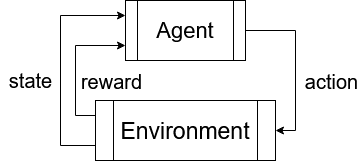
\includegraphics[scale=0.75]{RLEnv}
	\caption{A diagram of a typical Reinforcement Learning Environment.}
	\label{fig:RLEnv}
\end{figure}

\subsection{Taxonomy}

There are two main categories of RL algorithms, Model-Free, and Model-Based algorithms. The main distinguishing factor between these two categories is whether the agent has access to an environment model. A model of the environment could be a function that predicts the state transitions and rewards.

The model, within the Model-Based algorithm, is beneficial to the agent as it allows it to plan, thinking ahead, and evaluate the different action it could take—the result is a policy with experience from the different possible paths. An example is AlphaGo Zero, which utilizes the breathtaking Monte Carlo tree search (MCTS) algorithm. However, soldomly do we have access to the model function that the agent could use. In turn, if it wants to plane and formulate plans without access to the model, it would have to learn the model. One such algorithm is called MuZero, which can learn the rules of the games it plays, match the performance of AlphaZero, and achieve "state-of-the-art" performance in many Atari games. Leading to the two sub-categories under Model-Based Algorithms, Learned, and build-in model algorithms.

Under Model-Free algorithms, there are two sub-categories, Policy Optimization and Q-Learning based algorithms. The main differentiating factor between the two sub-categories is what the RL algorithm learns. In Policy Optimization-based algorithms, the algorithm directly learn a state to action mapping. The Q-learning based algorithms learns what is called a Q-function that satisfies the Bellman Equation. In other words, a Q-learning based algorithm will learn action from a set of actions by finding the maximum. Some algorithms that fall into Q-learning based algorithms include DQN, Dueling DQN TD3, DDPG, and Rainbow. Some algorithms that belong to the Policy Optimization category is A2C/A3C, TRPO, ACKTR, and PPO. 

Q-Learning based algorithms tend to be off-policy. Meaning, during training, these algorithms can use data from any point in the training processes. Off-policy algorithms train a different policy from generating the data, while On-policy algorithms train on the same policy generating the data.

\begin{figure}
	\centering
	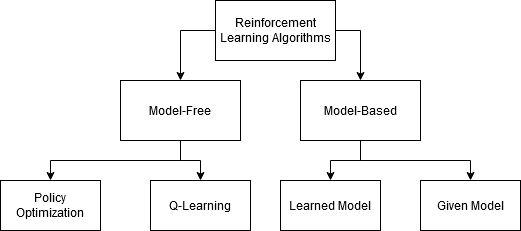
\includegraphics[scale=0.75]{Taxonomy}
	\caption{A diagram of Reinforcement Learning Algorithm's Taxonomy.}
	\label{fig:rltaxonomy}
\end{figure}

\subsection{Cross-Entropy Method}

The cross-entropy (CE) method is the second most straightforward algorithm to implement before the random algorithm. As the name implies, the random algorithm is just a random sampling of the available actions, and the CE method is only slightly more complicated to implement.

An intuitive explanation of the CE method is to create a distribution of episodes using their cumulative reward then train a neural network on the top $n$\% of the episodes. Over time, the neural network will learn the attributes of these best episodes. There are two variations to the CE method \cite{boer_kroese_mannor_rubinstein_2005}. The episode generation is entirely from random sampling, or the episode generation is form the latest policy. This algorithm is simple to implement but fails to learn from complicated environments. 

\begin{enumerate}[label=Step \arabic*:, itemsep=0mm]
	\item Generate a model with random weights.
	\item Run the environment for an $N$ number of episodes with current model, recording their cumulative reward, actions, and states.
	\item Only keep the top $n$\% of episodes with regard to their cumulative reward.
	\item Train the model on the remaining episodes.
	\item Go back to step 1, or exit when acceptable results have been achieved.
\end{enumerate}

\subsection{Q-Learning}

Q-Learning is a Model-free off-policy algorithm that uses tabulation. The Q in Q-Learning stands for quality, the quality of a particular action for a given state. $$Q:S\times A\rightarrow \mathbb{R}$$ A considerable part of off-policy algorithms and RL algorithms, in general, is the Bellman Equations. A table containing Q-Values is initiated, randomly or by some other means, and iterated according to the Bellman Equation for optimality. Where $A$ is the set of possible actions, 
\begin{equation}\label{eq:qupdate}
	Q_{t+1}(s_t, a_t)=Q_t(s_t, a_t)+\alpha \big(r_t+\gamma\max_{b\in A} Q_t(s_{t+1},b)-Q_t(s_t,a_t)\big).
\end{equation}
 The next action is chosen by $\max_{b\in A} Q_t(s_{t+1},b)$. Q-Learning tends to be combined with the $\epsilon$-greedy method to counteract and underfit and improve exploration. With the $\epsilon$-greedy method the chosen action becomes $$a_{\text{next}}=\begin{cases}\max_{b\in A} Q_t(s_{t+1},b) & \text{with probability }1-\epsilon \\ \text{random action}  & \text{with probability }\epsilon\end{cases}.$$

\subsection{Deep Q-Network (DQN)}

At a point, the number of state-action pairs, Q-values in the table becomes too large and too computationally expensive. A solution presented on a 2013 paper by DeepMind replaced this computationally expensive table with a Neural Network that maps the state and action to Q \cite{mnih_kavukcuoglu_silver_graves_antonoglou_wierstra_riedmiller_2013}. Unfortunately, just doing this replacement doesn't result in a stable algorithm for all environments. For instance, an environment with sparse rewards could result, when training, in non-convergence due to the imperfect initial Q representation. The $\epsilon$-greedy method helps in this respect, but there are many different optimizations, including Dueling and Double DQN, Prioritized Experience Replay, Noisy Nets, target networks, and others. This algorithm and it's variants works exceptionally well in Atari game environments, that have a large state space and small action space, where it uses a Convolutional Neural Network and the loss function optimized using SGD or ADAM, 
\begin{equation}\label{eq:dqnloss}
	L(s_t, a_t, r_t, s_{t+1})=\big(r_t+\gamma\max_{b\in A} Q_t(s_{t+1},b)-Q_t(s_t,a_t)\big)^2,
\end{equation} 
which is similar to the mean squared loss where $r_t+\alpha\max_{b\in A} Q_t(s_{t+1},b)$ is the target and $Q_t(s_t,a_t)$ is the prediction. Instead of using a table, this algorithm uses an experience replay buffer where past states, actions, rewards, and resulting states are stored and sampled to train the Neural Network.

Another massive problem with DQN is the fact that $Q(s_t, a_t)$ and $Q(s_{t+1}, a_{t+1})$ are only one step apart and, therefore, too similar. This similarity makes it too tricky for SGD or ADAM to train the Neural Network the mapping successfully. Here is where target networks come in. By separating the target and prediction Neural Network and allowing them to diverge, SGD and ADAM can train the target network; then, both network's parameters are periodically synchronized. The resulting Loss function is then $$L(s_t, a_t, r_t, s_{t+1})=\big(r_t+\gamma\max_{b\in A} \hat{Q}_t(s_{t+1},b)-Q_t(s_t,a_t)\big)^2.$$ Where $\hat{Q}$ is the Q-estimation \cite{mnih_kavukcuoglu_silver_rusu_veness_bellemare_graves_riedmiller_fidjeland_ostrovski_et}.

\begin{algorithm}
	\SetAlgoLined
	\DontPrintSemicolon
	Initialize experience replay queue $D$ with size $N$ \\
	Initialize Neural Network for $Q$ function with random weights \\
	Duplicate Neural Network $Q$ to $\hat{Q}$ \\
	episode $\leftarrow 1$\\
	\While{Reward has not converged}{
	Initialize environment $s\leftarrow e$ \\
	\For{$t=1,T$}{
		$a\leftarrow \begin{cases}\max_{b\in A} Q(s,b) & \text{with probability }1-\epsilon \\ \text{random action}  & \text{with probability }\epsilon\end{cases}$ \\
		$s_n, r\leftarrow e(a)$ Where $s$ is the state and $r$ is the reward\\
		$D.$append$(s, a, r, s_n)$\\
		$s\leftarrow s_n$\\
		Sample minibatch $(s, a, r, s_n)$ from $D$\\
		$y\leftarrow \begin{cases}r & t=T \\ r + \alpha max_{b\in A} \hat{Q}(s,b)& \text{otherwise}\end{cases}$\\
		Perform SGD or ADAM on $\big(y-Q(s_t,a_t)\big)^2$ with respect to $Q$'s parameters\\
		Every $N$ steps $\hat{Q}=Q$
	}}
	\caption{DQN with $\epsilon$-greedy and target network}\label{alg:dqn}
\end{algorithm}

\subsection{Rainbow}

DeepMind developed in 2017 the Rainbow algorithm \cite{hessel_modayil_hasselt_schaul_ostrovski_dabney_horgan_piot_azar_silver_et}, which incorporates six improvements to the DQN version publish in their 2015 paper \cite{mnih_kavukcuoglu_silver_rusu_veness_bellemare_graves_riedmiller_fidjeland_ostrovski_et}, which itself incorporates some improvements like target networks to the vanilla paper in 2013 \cite{mnih_kavukcuoglu_silver_graves_antonoglou_wierstra_riedmiller_2013}. This algorithm really is a culmination of various improvements to DQN \cite{hessel_modayil_hasselt_schaul_ostrovski_dabney_horgan_piot_azar_silver_et}. These improvements include:
\begin{enumerate}[itemsep=0mm]
	\item Double Q-Learning
	\item Prioritized Experience Replay
	\item Dueling Network
	\item Multi-step learning
	\item Distributional RL
	\item Noisy Nets
\end{enumerate}

Double Q-Learning is an update to the Q update equation~\ref{eq:qupdate} that fixes a problem where the Q-values are overestimated for some actions; Hado van Hasselt et al. showed this overestimation in its presentation of Double Q-Learning where the author proved that this overestimation exists, more generally, due to any inaccuracy during learning. This problem is due to the max step in equation~\ref{eq:qupdate} and  is addressed by decoupling the max step from action selection. This decoupling, in Deep Q-Learning, results in two separate Q NN models, $$Q_1(s_t, a_t)\leftarrow Q_1(s_t, a_t)+\alpha (r_t+\gamma Q_2(s_{t+1}, \max_{b\in A}Q_1(s_{t+1}, b)) - Q_1(s_t, a_t)).$$ This results in the loss function $$L(s_t, a_t, r_t, s_{t+1})=(r_t+\gamma Q_2(s_{t+1}, \max_{b\in A}Q_1(s_{t+1}, b)) - Q_1(s_t, a_t))^2 \cite{hasselt_guez_silver_2015}.$$

The Prioritized Experience Replay modification tackles another part of the DQN algorithm, the Experience Replay. The regular experience replay, in implementation, would be a Queue with random access and a maximum number of elements where if the Queue reaches capacity, it would merely pop items. Some of the items thrown away have embedded important state-action information and, also, the sampling of data for training the Q models is entirely random, leading the model to learn wrong information. It makes sense to create a replay that priorities essential samples when sampling to train and only throw away the unimportant samples; the first is what the Prioritized Experience Replay achieves. Instead of sampling in a uniform random fashion, it samples with probability pt relative to the last encounter with a prioritization value. Tom Schaul et al. presents two different functions for this prioritization value, one is TD-Error or temporal difference error, and the other is a stochastic sampling method that interpolates between the TD-Error and uniformly random. Rainbow, however, only uses TD-Error \cite{schaul_quan_antonoglou_silver_2016}. $$p_t\propto \big[r_t+\gamma_{t+1}\max_{b\in A}Q_1{s_{t+1}, b}-Q_2(s_t, a_t) \big]^\omega$$ Where $\omega$ is a hyper-parameter for the probability distribution. New additions to this replay have $p_t=1$. 
The typical way of implementing this replay would be a Priority Queue with random access, but because large portions of the queue probabilities need to be updated, a Segment Tree is optimal. Summing a portion of the Queue requires $O(n)$ complexity while a Segment Tree's complexity is $O(\log n)$.


The third improvement is Dueling Networks. This improvement requires introducing the advantage, which is a value obtained by subtracting the Q-value by that state's value, 
\begin{equation}\label{eq:advantage}
	A(s,a)=Q(s,a)-V(s).
\end{equation}
 Ziyu Wang et al. proposes instead of estimating the Q-value directly, using a Neural Network to estimate the Advantage and the Value of the function and calculate the Q-value from that. Intuitively one would try to calculate the Q-value via equation~\ref{eq:advantage} by reformulating it to $Q=V+A$, but this would be a mistake. After summing the value and the advantage when training, the resulting Q-value is "unidentifiable." The value and the advantage are not recoverable from this Q-value, leading to bad performance. The solution is to zero the advantage for the chosen action, $$Q(s, a)=V(s)+A(s, a)-\frac{\sum_{b\in A} A(s, b)}{n_{\text{actions}}}.$$ Instead of having two CNNs or NNs to estimate the value and estimate the advantage, Rainbow uses a backbone CNN with a two-prong NN; one prong estimates the value, and the other estimates the advantage \cite{wang_frietas_lanctot_2015}.
 
Multi-step learning has initially been an expansion of Q-Learning, where instead of calculating a single-step Q-value, the rewards for n-steps are used and accumulated for the n-step Q-value \cite{sutton_1988}. Similarly, for Deep Q-Learning, this n-step is instead an approximation. The discounted reward function would then be $$r_t^{(n)}\equiv \sum_{k=0}^{n-1} \gamma_t^k r_{t+k+1}$$ and the resulting loss function is $$L(s_t, a_t, r_t, s_{t+1})=(r_t^{(n)}+\gamma^{(n)} Q_2(s_{t+1}, \max_{b\in A}Q_1(s_{t+1}, b)) - Q_1(s_t, a_t))^2 \cite{hessel_modayil_hasselt_schaul_ostrovski_dabney_horgan_piot_azar_silver_et}.$$
 
In Distributional Reinforcement Learning, the next improvement to Rainbow the returns' distribution is learned instead of the expected reward. The bellman equation is replace by the distributional bellman equation. Here instead of a single expected reward is created from the distributional model but a series of atom that represent a distribution. These atoms are defined by $$z_i=v_{\min} +(i-1)\frac{v_{\max}-v_{\min}}{N_{\text{atoms}}-1}.$$ Where $v_{\max}$ is the largest possible return of the distribution, $v_{\min}$ is the smallest possible return of the distribution, $N_{\text{atom}}$ are the number of atoms to use in the distribution \cite{bellemare_dabney_munos_2017}. 

The last improvement to the DQN function expands the exploration done by the network freeing it from the $\epsilon$-greedy method and embedding this exploration within the Q-approximating model itself. A DQN Neural Network model's basic anatomy consists of an initial series of Convolutional Layers with the typical RELU layers in between. This series is then followed by a flattening of the tensor and a Feed-Forward Neural Network. Following this series of Convolutional Layers and a tensor's flattening, the following Neural Network's layers are replaced with Noisy Layers, $$\vec{a}=(\vec{b}+W\vec{x})+(\vec{b}_{\text{noisy}}\odot \epsilon^b +(W_{\text{noisy}}\odot \epsilon^w)\vec{x}).$$ Where $\vec{b}_{\text{noisy}}$ and $W_{\text{noisy}}$ are a trainable vector and matrix whose initial values are random, as are $\vec{b}$ and $W$. $\epsilon^b$ and $\epsilon^W$ are a random vector and weight generated from a normal distribution \cite{fortunato_azar_piot_menick_osband_graves_mnih_munos_hassabis_pietquin_et}. 

\subsection{REINFORCE}\label{subsec:reinforce}

An alternative to Q-Learning methods is Policy Optimization methods. These method's goal is to optimize the probabilities of actions in order to have higher returns. Since these methods rely directly on optimizing the policy instead of recording the state-action pair, it is more efficient when learning environments with continuous actions and continuous states.

A  performance measure is required here and a symbol that stands for a policy's parameters, $\theta$. This performance measure is defined as $J$ and is a function of the policy parameter, $J(\theta)$. Similarly, the policy's notation evolves to a function also with regards to its policy parameters. These Policy Optimization algorithms aim to optimize the performance; if SGD is used to optimize $J(\theta)$, $$\theta_{t+1}=\theta_t+\alpha \nabla J(\theta_t).$$ $J$ is defined as $$J(\theta)\equiv v_{\pi_{\theta}}(s_0).$$ $v_{\pi_{\theta}}$ is the value of a state with regard to the policy, $\pi_{\theta}$. Notice $J$ depends also on the state, this changes to the policy's parameters difficult. The policy gradient theorem fixes by separating the policy; it is defined as $$\nabla J(\theta)\propto \sum_s \mu(s) \sum_a q_\pi (s, a)\nabla_{\theta} \pi (a|s, \theta).$$ Where $\mu(s)$ is the on-policy distribution under $\pi$, 

In the Vanilla Policy Gradient (VPG) or Policy Gradient (PG) method, Vanilla, because it has no modifications, the algorithm samples actions according to the latest policy and over time, while at the start of training is almost entirely random, over time becomes less random. A con to this method is, it does tend to get stuck in a local optimum.

One of the simplest is REINFORCE; it is a Monte-Carlo version of the Policy Gradient Algorithm. There is, however, more than one version of this algorithm, each implements an improvement over the vanilla REINFORCE algorithm, but they all, by Monte-Carlo methods, rely on an estimated return to update the policy's parameters. Using the policy gradient theorem as a basis
\begin{align*}
	\nabla J(\theta)&\propto \sum_s \mu(s) \sum_a q_\pi (s, a)\nabla_{\theta} \pi (a|s, \theta) \\
	&=\mathbb{E}_\pi \bigg[\sum_a q_\pi(s_s, a)\nabla_\theta \pi(a|s_t, \theta)\bigg].
\end{align*} After manipulation, this equation yields to the estimate of $\nabla J(\theta)$ ,$$\nabla J(\theta)=\mathbb{E}\bigg[G_t \frac{\nabla_\theta \pi(a_t|s_t, \theta)}{\pi(a_t|s_t, \theta)}\bigg]\bigg|a_t\in \text{possible actions},$$ which, when plugging into the parameter update, we get the following equation, $$\theta_{t+1}=\theta_t+\alpha G_t\frac{\nabla_\theta \pi(a_t|s_t, \theta)}{\pi(a_t|s_t, \theta)}=\theta_t + \alpha G_t \nabla_\theta \ln \pi(a_t|s_t, \theta).$$ Notice how the identity $\frac{\nabla x}{x}=\nabla \ln x$ is used.

\begin{algorithm}
	\SetAlgoLined
	\DontPrintSemicolon
	\KwIn{A policy $\pi(a|s, \theta)$ with initialized parameters $\theta$}
	\While{Reward has not converged}{
		Run environment for a single episode with $D=\{(s_0, a_0, r_1), \dots, (s_{T-1}, a_{T-1}, r_T)\}$\\
		Calculate $G_t$ for every step in the episode via equation~\ref{eq:discountedreward}\\
		\For{$d\in D$}{
			$\theta\leftarrow\theta+\alpha G_t \nabla_\theta \ln \pi(a_t|s_t, \theta)$
		}
	}
	\caption{REINFORCE Algorithm}
\end{algorithm}

An improvement to REINFORCE integrates a baseline function. This baseline function becomes very important, especially in the A2C algorithm. The problem that the baseline function mitigates is its high variance. An example of this variance can be seen with the trajectory that results in $\nabla_\theta \ln \pi(a|s, \theta)=[0.4, 0.6, 0.8]$ and $G=[255, 300, 350]$ then the variance of their component-wise product is calculated to 
\begin{align*}
	Var(\nabla_\theta \ln \pi(a|s, \theta)\times G)&=Var([0.4\times 255, 0.6\times 300, 0.8\times 350])\\
	&=Var([102, 180, 280])\\
	&=7961.3.
\end{align*} The objective function with the baseline function is $$\nabla J(\theta)=\mathbb{E}[(G_t-b(s_t))\nabla_\theta \pi (a_t|s_t, \theta)].$$ If we then let $b(s_t)=450$ then the calculated variance will then be $41.34$. In Algorithm~\ref{algo:REINFORCEBASELINE}, both $\alpha_w$ and $\alpha_\theta$ are two separate learning rates, $w$ is a weights vector. The function $\hat{v}$ can be as simple as $\hat{v}(s, w)=w$.

\begin{algorithm}\label{algo:REINFORCEBASELINE}
	\SetAlgoLined
	\DontPrintSemicolon
	\KwIn{A policy $\pi(a|s, \theta)$ with initialized parameters $\theta$}
	\KwIn{A state-value function that is parameterized $\hat{v}(s, w)$}
	\While{Reward has not converged}{
		Run environment for a single episode with $D=\{(s_0, a_0, r_1), \dots, (s_{T-1}, a_{T-1}, r_T)\}$\\
		Calculate $G_t$ for every step in the episode via equation~\ref{eq:discountedreward}\\
		\For{$d\in D$}{
			$\delta\leftarrow G_t - \hat{v}(s_t, w)$\\
			$w\leftarrow w + \alpha_w \gamma^t \delta \nabla \hat{v}(s_t, w)$\\
			$\theta\leftarrow\theta + \alpha_\theta \gamma^t \delta \nabla \ln \pi(a_t, s_t, \theta)$
		}
	}
	
	\caption{REINFORCE Algorithm w/ Baseline}
\end{algorithm}

\subsection{DDPG}

Deep Deterministic Policy Gradient (DDPG) is interesting as it is an adaptation of DQN for environments with continuous action spaces. One of the problem in using DQN for environments with continuous action spaces has to do with the fact that Q-Learning considers a finite number of actions but continuous action spaces have an infinite number of actions. More specifically the $\max$ function used to calculate the loss, Equation~\ref{eq:dqnloss}, is computationally expensive when there are an infinite number of possible actions to choose from. DDPG fixes this by, instead of trying to find the action with the maximum Q-value, having a policy estimate an action which will result in a large Q-value, $max_{b\in A} Q(s,b)\approx Q(s, \pi(s))$ \cite{lillicrap_hunt_pritzel_heess_erez_tassa_silver_wierstra_2015}.

This is then combined with some tricks used in DQN, Replay Buffers and Target Networks, results in the DDPG algorithm. The loss function, with Target Networks, is then $$L(s_t, a_t, r_t, s_{t+1})=\big(r_t+\gamma \hat{Q}_t(s_{t+1},\pi(s_{t+1}))-Q_t(s_t,a_t)\big)^2.$$

\subsection{A2C/A3C}

Asynchronous Advantage Actor Critic (A3C) and A2C, a derivative of A3C that is synchronous, is an algorithm first described in a 2016 paper, \cite{mnih_badia_mirza_graves_harley_lillicrap_silver_kavukcuoglu_2016}. This algorithm, fundamentally, is an extension of the REINFORCE with baseline algorithm. It also combines Q-learning via the advantage function, equation~\ref{eq:advantage}.

\subsection{Trust Region Policy Optimization (TRPO)}

TRPO, \cite{schulman_levine_mortiz_jordan_abbeel_2015}, is the precursor to the PPO algorithm but weirdly is more complicated. TRPO is an improvement over the PG method. It fixes a big problem in the PG method, where it becomes overconfident and learns the wrong behaviors. Notice from subsection~\ref{subsec:reinforce} how the REINFORCE method, and in turn, the PG method, are first-order methods and are therefore unable to take into account the second-order curvature while maximizing the reward. If REINFORCE makes a step in the rewards graph that results in worse performance, it then continues from this worse state. Another fault with REINFORCE happens because the entire trajectory for an episode is required before the policy is update, resulting in low sample efficiency. 

TRPO improves PG by integrating the MM algorithm, otherwise called the Majorize-Minimization algorithm, which finds substitute, lower or higher bound functions and is an iterative algorithm. It then optimizes based on this function, which guarantees optimization \cite{lange_2007}. In the MM algorithm, a function $g(\theta|\theta_m)$ is the minorize of the function $f(\theta)$ when 
\begin{align*}
	g(\theta|\theta_m)&\leq f(\theta) &\text{for all }\theta\\
	g(\theta_m|\theta_m)&=f(\theta_m). 
\end{align*} Then, to maximize the reward, a minorize function is found and maximized, which produces the next point, $\theta_{m+1}$, from which to maximize. Further, it goes that every further point's reward is either greater or equal to the previous point. The second improvement to the PG method is a change from the line optimization, where Gradient Descent chooses a direction, and takes a fixed-sized step, whereas, in Trust Region, the algorithm first calculates the maximum sized step, after which it finds the optimal step within that region to take.

It samples actions according to the latest policy, firstly in a random manner. As time goes on the algorithm learns, the actions sampled become less random. Of course, this can mean the algorithm is stuck in a local maxima. This progression, of course, also means the algorithm can get stuck in a local maximum. In these Trust Region optimization algorithms, the quadratic Taylor expansion approximates the objective function \cite{nocedal_wright_2006}. \begin{align*}
	\bar{f}(x)&\approx f(x) \\
	&=f(c)+\nabla J(c)^T(x-c) + \frac{1}{2!}H(c)(x-c)
\end{align*} here th $J$ is the Jacobian matrix, the first-order part, and $H$ is the Hessian matrix, the second-order part. The trust region, the maximum possible step, is typically calculated as $||x-c||_2\leq \delta$, a hypersphere, where $\delta$ is a threshold parameter and $c$ is a constant. Note, the farther $x$ is from $c$, the less accurate the approximation.

This algorithm's complexity steps from the required calculation of the approximation of the inverse Hessian matrix, a set of second-order partial derivatives, of an average Kullback-Leibler (KL) divergence; hence, this is a second-order algorithm. Nonetheless, this algorithm gives monotonic improvement and is one of the first on-policy algorithms that train policies with many parameters. 

\subsection{Proximal Policy Optimization (PPO)}

PPO differs from TRPO as PPO is a first-order method, but like TRPO, it aims to take the broadest possible step without degrading performance.